\documentclass[10pt,twocolumn,letterpaper]{article}
\usepackage{graphicx}
\usepackage{amsmath}
\usepackage{amssymb}
\usepackage{booktabs}
\usepackage{nicefrac}
\usepackage{algorithm}
\usepackage[algo2e]{algorithm2e} 
\usepackage{multirow}
\usepackage[pagebackref,breaklinks,colorlinks]{hyperref}

% Support for easy cross-referencing
\usepackage[capitalize]{cleveref}
\crefname{section}{Sec.}{Secs.}
\Crefname{section}{Section}{Sections}
\Crefname{table}{Table}{Tables}
\crefname{table}{Tab.}{Tabs.}

\begin{document}
\nocite{*}
\author{Tamo steve}
\maketitle
learning, and cosine similarity loss for normal estimation:
\begin{equation}
\left\{
    \begin{array}{ll}
        \mathbf{l}_{mask}  = ||\mathbf{M} - \mathbf{\hat{M}}||_{1}\\
        \mathbf{l}_{xyz} = \mathbf{M} \odot ||\mathbf{M}_{xyz} - \mathbf{\hat{M}}_{xyz}||\\
        \mathbf{l}_{normal} = 1 - \langle\mathbf{n},\mathbf{\hat{n}}\rangle
    \end{array}
\right.
\end{equation}
where $\odot $indicates the Hadamard product of element-wise
multiplication, and $\langle\bullet,\bullet\rangle$ denotes the dot product.
%% Here goes your code

\section{Experimental Results}
The motivation of our proposed pipeline is to show the
advantage of leveraging pixelwise physical priors from polarised light (a.k.a. RGBP) for accurate 6D pose estimation
of photometrically challenging objects - for which \textbf{RGB-} only and \textbf{RGB-D} methods often fail. For this purpose, we
train and test \textbf{PPP-Net} with different modalities first on two
exemplary objects with very different level of photometric
complexity, i.e. a plastic cup, and a photometrically very
challenging, reflective and textureless stainless steel cutlery
knife. As detailed later, we find that polarimetric information yields significant performance gain for photometrically
challenging objects.

\subsection{Polarimetric Data Acquisition}
    To evaluate our pipeline we leverage 6 models from the
PhoCal [1] category-level pose estimation dataset which
comprises 60 household objects with high-quality 3D
models scanned by a structured light 3D stereo scanner
(EinScan-SP 3D Scanner, \textbf{SHINING 3D Tech. Co., Ltd.},
Hangzhou, China). The scanning accuracy of the device is
$\leq 0.05$ mm which allows for highly accurate models. We
select the models cup, teapot, can, fork, knife, bottle with
increasing photometric complexity which we illustrate in
Fig. 6. The last three models do not include texture due to
their surface structure. The 3D scanning has been done with
a vanishing 3D scanning spray that made the surface temporarily opaque. To acquire \textbf{RGB-D} images, we use a direct Time-of-Flight (dToF) camera, intel RealSense LiDAR Camera L515 (intel, Santa Clara, California, USA), which
captures RGB and Depth data at 640x480 pixel resolution. RGBP is acquired using the polarisation camera Phoenix 5.0 MP PHX050S1-QC comprising a Sony IMX264MYR CMOS (Color) Polarsens sensor (LUCID Vision Labs, Inc., Richmond B.C, Canada) through a Universe Compact CMount 5MP $2/3”$ 6mm $f/2.0$ lens (Universe, New York, USA) at 612x512 pixel resolution. Both cameras are mounted jointly to a KUKA iiwa (KUKA Roboter GmbH, Augsburg, Germany) 7 DoF robotic arm that guarantees a positional reproducibility of $\pm0.1 mm$. Intrinsic and extrinsic calibration is performed following the standard pinhole camera model [59] with five distortion coefficients [22]. For pose annotation, we leverage the mechanical pose annotation method proposed in PhoCal [1] where the robotic manipulator is used to tip the object of interest and extract a point cloud. This point cloud is consecutively aligned to the 3D model using ICP [6] to allow for highly accurate pose labels even for photometrically challenging objects. We plan a robot trajectory and use this setup to acquire four scenes with four different trajectories each and utilise a total of 8740 image sets for the dataset.
\subsection{Experiments Setup}
\textbf{Implementation Details}. We initially refine an off-theshelf detector Mask RCNN [19] directly on the polarised images I0 to provide useful object crops on our data (as is needed for the RGB-only benchmark and ours). We follow
similar training/testing split strategy as commonly used for the public datasets [9], and employ $≈ 10\%$ of the RGBP images for training and $90\%$ for testing. We train our network end-to-end with Adam optimiser [33] for 200 epochs.
The initial learning rate is set to $1e-4$, which is halved every 50 epochs. As the depth sensor has a different field of view and is placed beneath the polarisation camera on a customised camera rig, the RGB-D benchmark split differs
from the RGB training/testing split.

\textbf{Evaluation Metrics}. To establish our proposed novel 6D pose estimation approach, we report the pose estimation accuracy per object as the commonly used average distance (ADD) and its equivalent for symmetrical objects (ADDS) [23] for different benchmarks. For the surface normal estimation, we calculate the mean and median errors (in degrees) and the percentage of pixels where the estimated normals vary less than $11.25^\circ$, $30^\circ$ and $30^\circ$ from the ground truth. We additionally give valuable insights into our proposed pipeline by performing detailed ablations on the input modalities, the fusion of complementary modalities, and the
effect of explicit learning of physically plausible geometric
information and its effect on pose prediction accuracy (see Tab. 1), and discuss limitations of our proposed approach.
\subsection{PPP-Net}
Here, we perform a series of experiments to study the influence of the input modality on the pose estimation accuracy (compare Tab. 1), where we specifically analyse the influence of polarimetric image information for the task of $6D$ object pose estimation. We demonstrate that our network with RGBP input performs at the state-of-the-art level
\begin{figure}[H]
    \centering
    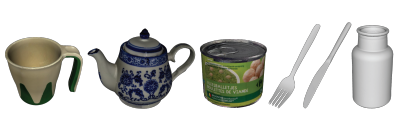
\includegraphics{image/Capture d'écran_20230110_145736.png}
    \caption{3D Models. Test objects with increasing photometric complexity (left to right). Three objects have no texture in as they are reflective (cutlery) or transparent (bottle).}
    \label{fig:my_label}
\end{figure}
\renewcommand{\thesection}{\Alph{section}}
\section{ Physical Priors}
We use physical priors as inputs in our network to improve the estimated 6D pose of an object. These priors form relations between polarisation properties and azimuth and zenith angle of the surface normal, which serves as geometric cues orthogonal to color information. We calculate the physical priors under the assumption of either specular or diffuse reflection.

To recover the azimuth and zenith angle of the surface
normal, we present the calculation for solving the unknowns
of \cref{eq:SLAMequa}.

A polarimetric camera registers intensity behind four linear polarisers with angles $0^\circ, 45^\circ, 90^\circ, 135^\circ,$ which depends on unpolarised intensity \textit{I}, degree of polarisation $\rho$, and angle of polarisation $\phi$:
\begin{equation}
    \textit{I}_{\rho pol} = \textit{I}_{un} \cdot (1 + \phi\cos(2(\phi - \rho_{pol})))
    \label{eq:SLAMequa}
\end{equation}

\cref{eq:SLAMequa} can be re-written as:
\begin{equation}
    \textit{I}_{\rho pol} = \underbrace{\left(\begin{array}{c c c} 
                                                1\\
                                                \cos(2\rho_{pol})\\ 
                                                \sin(2\rho_{pol}) 
                                                \end{array}
                                                \right)^T}_{\beta^{T}}\underbrace{\left(\begin{array}{c c c} 
                                                \textit{I}_{un}\\
                                                \cos(2\rho_{pol})\\ 
                                                \sin(2\rho_{pol}) 
                                                \end{array}
                                                \right)}_{x}
    \label{eq:SLAMequa}
\end{equation}

{\small
\bibliographystyle{IEEEtran}
\bibliography{references}
}

\end{document}

